\chapter{Simulation Framework}
\label{chap:sim}
\section{Overview}

A simulation allows for the modeling and testing in a physics environment \cite{vzlajpah2008simulation}; this allows for analysis and measurements of controllers and their execution in different environments for robotics systems simulation. This feature makes it an ideal tool for the development of robotic systems. Simulation allows for controllers to be designed and tested. The simulation framework presented here is used to develop different controllers for the LARRE exoskeleton. All the controllers will be tested on the simulated LARRE model. Due to the current limitation and of AMBF all the controllers are tested with the hip of the exoskeleton fixed in space with no interaction with the ground. With further development of AMBF it is possible to adapt the controller methods present in this dissertation for ground level walking at slow speeds. 

The Asynchronous Multi-Body Framework (AMBF) was used to simulate LARRE \cite{AMBF}. This framework was developed in the WPI AIM lab. 
AMBF is a real-time dynamic simulation environment for robotics systems and uses the Robotic Operating System (ROS)\cite{quigley2009ros} as a middleware for external user control. It allows for a wide range of simulated robotics systems, including surgical robots, exoskeletons, cars, and serial manipulators. The robots are defined using AMBF description files that utilize the YAML\footnote{https://yaml.org/} format. The file describes the robot's links and joints. AMBF contains rigid body objects, sensors, and actuators. These different object types can be combined to create various robotic systems with complicated structures and sensing capabilities. 
 
 
 The AMBF simulation environment runs at $1000Hz$; this allows for control loops designed to react to and control the exoskeleton.  AMBF contains built-in Python and C++ clients that handle the ROS communication between the user and the simulation environment. This client allows for bidirectional communication to get and set the joint angles and model state and set joint torques. The joint angles, velocities, and efforts are controlled individually or together. The joint effort is the primary control type used in this paper. 
 
Robotic controllers typically require knowledge of the systems' dynamics being controlled \cite{piltan2012design}; this includes the properties of the links and the relationship of the joints. The dynamics model allows for the cancellation of the non-linear terms and gravity compensation. The discrepancy between the simulation model and the control model can lead to the instability of the controller. 
 
 While AMBF provides a simulation environment and a method to communicate with the model, there was no method to control the robots. A control interface was developed to calculate control inputs and the dynamics of a simulated model. This control architecture is discussed below. In addition, due to how relatively new this simulation package is, several contributions were made to the package to fix the functionality. All of the changes have been included in the open-source build of the simulation. The feature enhancements include:
 \begin{itemize}
     \item Fixed bugs to the communication client
     \item Feature enhancements for accessing the model state
     \item Feature enhancements for accessing the sensors 
     \item Fixed bugs for the joint effort control
     \item Fixed bugs in pointclouds for the depth cameras
 \end{itemize}
 
 \section{LARRE AMBF Model}
 
 The LARRE exoskeleton was modeled in Blender \footnote{https://www.blender.org}, which is used to generate the ADF (AMBF description file) file for AMBF. The Blender LARRE model is shown in \autoref{fig:blender}. The dynamic properties of the bodies were calculated using SolidWorks. The hip of the exoskeleton was set as the root of the model—each leg has 3 DoF: the hip, knee, and ankle. Crutches were added to the system to support the upper body. A human model was added to the model to simulate a person wearing the exoskeleton. The human joints were made co-linear to the exoskeleton; however, they are treated as separate and independent joints. The mass of each of the segments was based on $80kg$ North American male \cite{BMI} \cite{drillis1964body}.
 
 \begin{figure}[h]
     \centering
     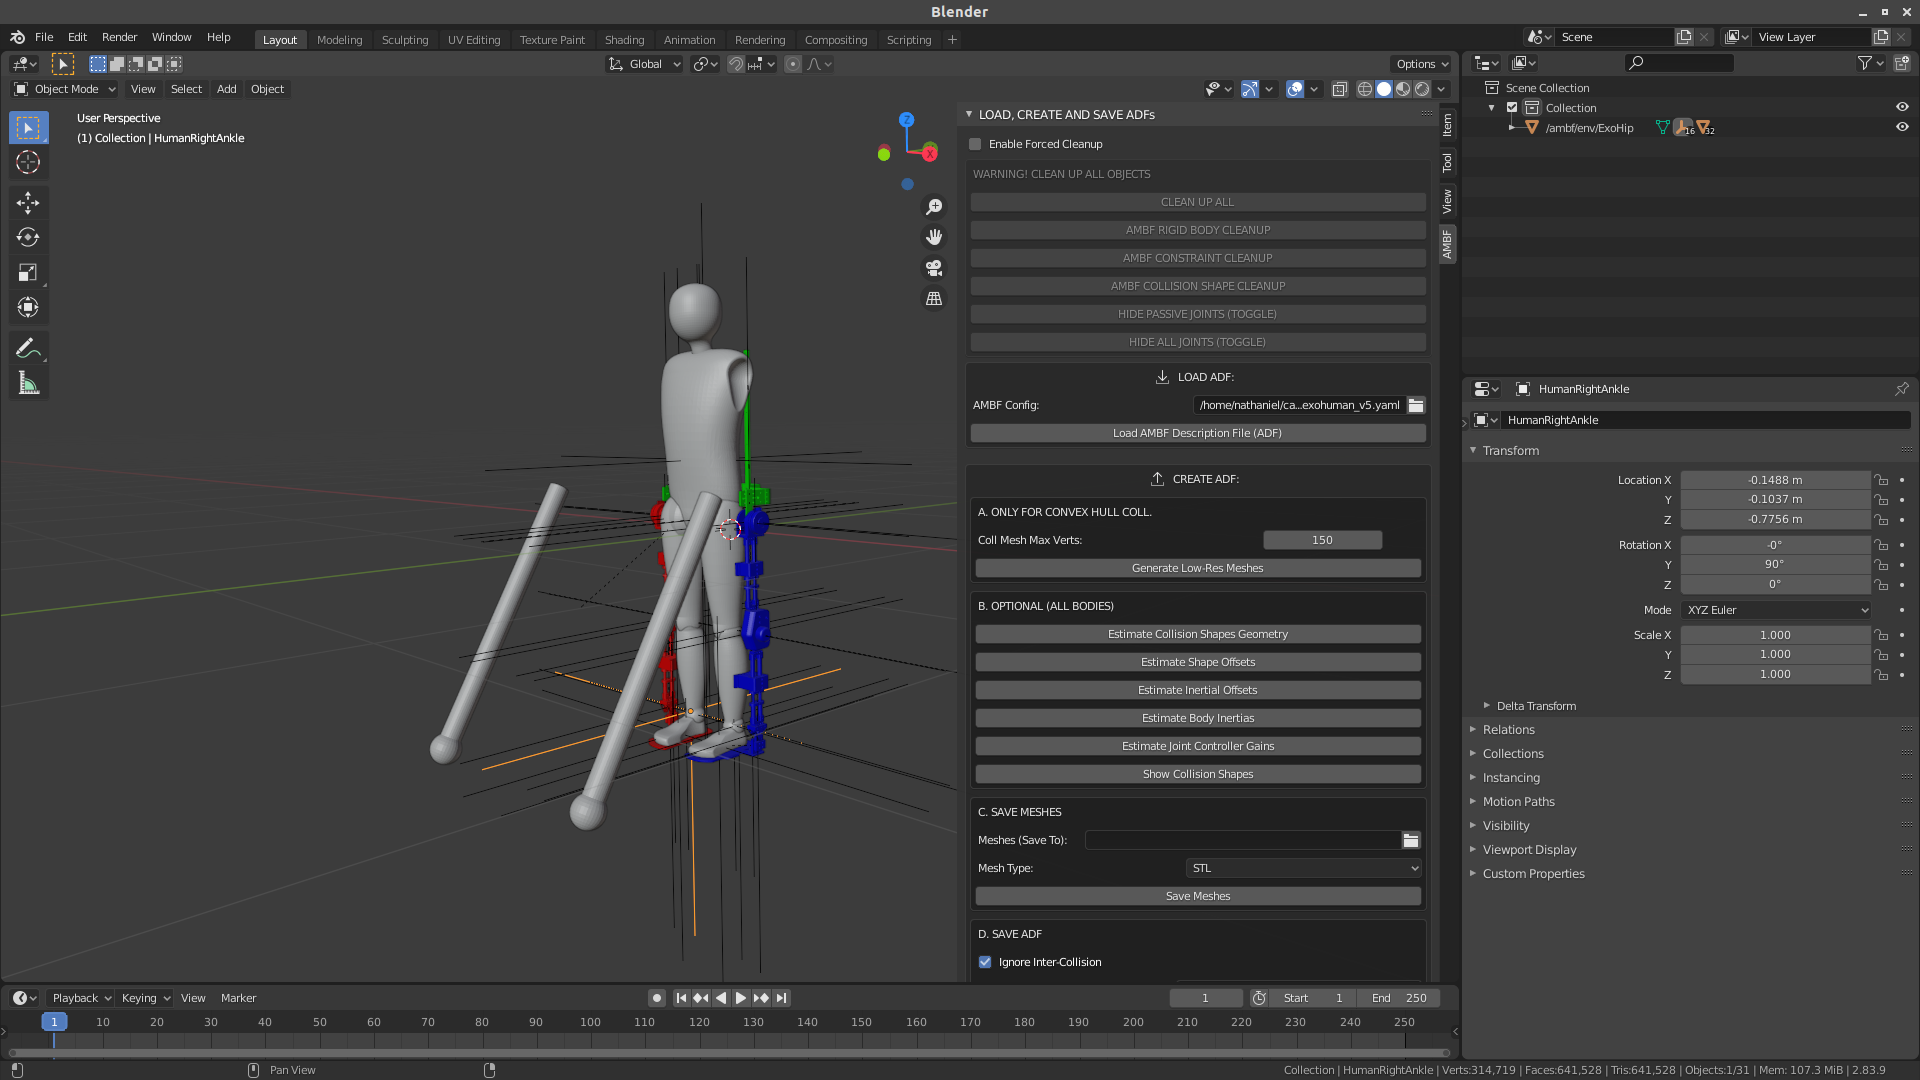
\includegraphics[scale=0.2]{images/sim/blender.png}
     \caption[Blender Model of LARRE]{Creating the AMBF model of LARRE using the ambf\_addon tool}
     \label{fig:blender}
 \end{figure}
 
 
 The \textit{exohuman} model consists of both the human and LARRE model. It has a total of 12 active DoF:

\begin{enumerate}
  \item Exoskeleton Left Hip
  \item Exoskeleton Left Knee
  \item Exoskeleton Left Ankle
  \item Exoskeleton Right Hip
  \item Exoskeleton Right Knee
  \item Exoskeleton Right Ankle
  \item Human Left Hip
  \item Human Left Knee
  \item Human Left Ankle
  \item Human Right Hip
  \item Human Right Knee
  \item Human Right Ankle
\end{enumerate}

 
 Each joint can be independently controlled and measured. The joints provide their position, velocity, and effort to the Python client, allowing the joint states to be measured and used for control. The \textit{exohuman} model consists of both the human and LARRE model. This is the first bipedal exoskeleton model that has been built for use in AMBF. Until now, the primary use of AMBF has been used to simulate robotic surgical systems. The exoskeleton adds several layers of difficultly since it is not a static system. Additionally, since the human model is connected to the exoskeleton, the two model segments can interact. The effort supplied by the human model will affect the joints of the exoskeleton; this allows for the testing of cooperative controllers, which is critical for developing the exoskeleton controller. The human effort is accounted for in the dynamic of the system.  
 
 
 Several sensors were built into LARRE to measure the joint states and the environment, including the joint positions and velocities. This is shown in \autoref{fig:simwalkingTraj}, where LARRE's joint positions and the human joint positions are compared to the desired trajectory.  \author{fig:simwalkingtorque} shows the torques over the same walking trajectory. As expected, the human and exoskeleton follow the same trajectory due to the joints of the human and exoskeleton being co-linear.  Similarly, \autoref{fig:simwalking} shows LARRE being controlled from a stand to sit cycle motion.
 
 
 \begin{figure}[h!]
    \begin{subfigure}{0.5\textwidth}
        % \hspace*{-1cm} 
        \centering
        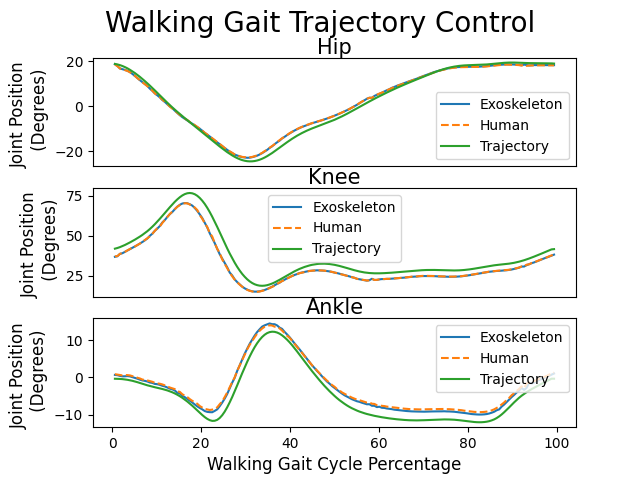
\includegraphics[scale=.5]{images/sim/walkjoints.png}
        \caption{Comparing the actual joint angle vs the desired joint angles}
        \label{fig:simwalkingTraj}
    \end{subfigure}
    \begin{subfigure}{0.5\textwidth}
        % \hspace*{-1cm} 
        \centering
        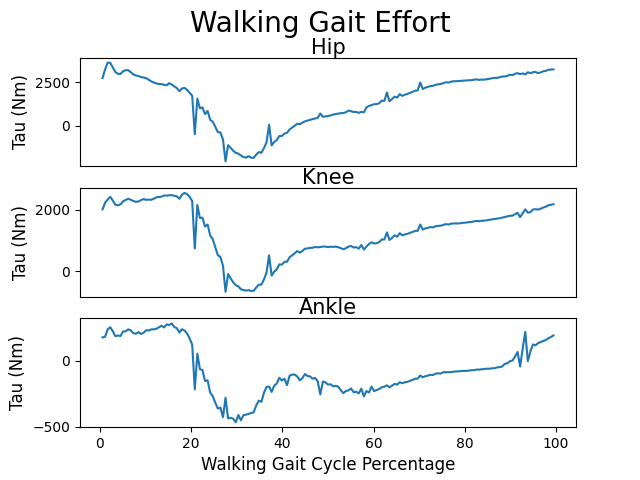
\includegraphics[scale=.5]{images/sim/walktau.png}
        \caption{The toques over a gait cycle for each of the joints}
    \label{fig:simwalkingtorque}
\end{subfigure}
    \caption[LARRE Simulation Gait Kinematics]{LARRE being controlled through a walking gait cycle}
    \label{fig:simwalking}
\end{figure}
 
 
 
  \begin{figure}[h!]
    \begin{subfigure}{0.5\textwidth}
        % \hspace*{-1cm} 
        \centering
        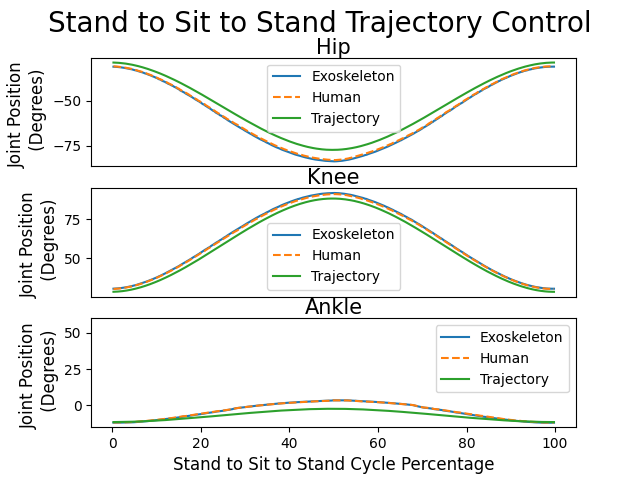
\includegraphics[width=\textwidth]{images/sim/standsitstandjoints (1).png}
        \caption{Trajectory comparison a stand to sit back to stand position}
        \label{fig:simsit2standTraj}
    \end{subfigure}
    \begin{subfigure}{0.5\textwidth}
        % \hspace*{-1cm} 
        \centering
        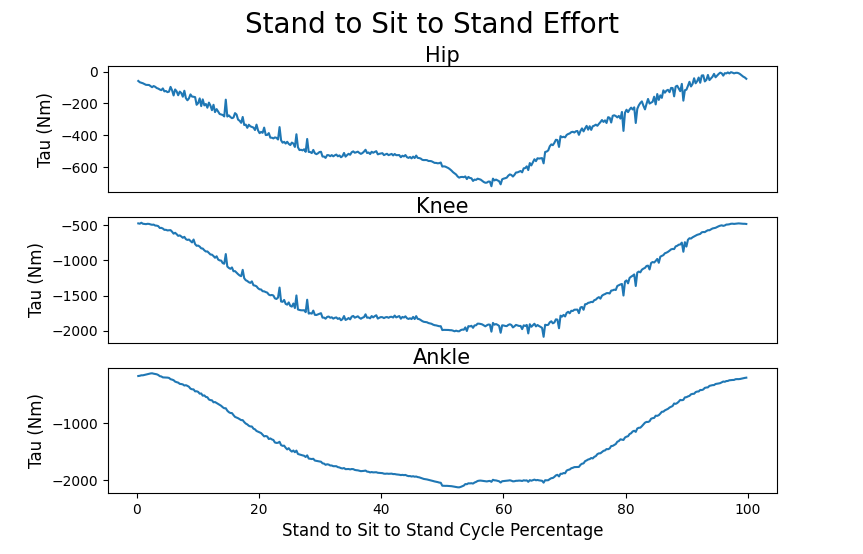
\includegraphics[width=\textwidth]{images/sim/standsitstandtau.png}
        \caption{The toques for stand to sit back to stand position }
    \label{fig:simsit2standtorque}
\end{subfigure}
    \begin{subfigure}{0.5\textwidth}
        % \hspace*{-1cm} 
        \centering
        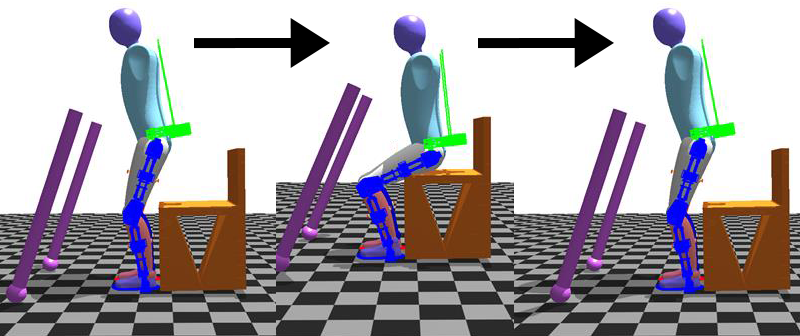
\includegraphics[scale=.5]{images/sim/sit_to_stand2 (1).png}
        \caption{Exoskeleton moving through the desired motion}
    \label{fig:sit2stand}
\end{subfigure}
    \caption[LARRE Simulation standing to sit motion]{LARRE being controlled through a stand to sit to stand cycle}
    \label{fig:simwalking}
\end{figure}
 
 
 
 Two LIDARs were equipped to LARRE, one on each side; they have a $45^{\circ}$ span and a $1.5m$ range. The sensor array can detect objects in the environment. \autoref{fig:exostair} shows the LIDARs measuring a staircase. A depth camera is attached to the exoskeleton hips. The camera produces a rich 3D point cloud, which is transformed into the LARREs frame using the PointCloudLibrary \cite{Rusu_ICRA2011_PCL}.  \autoref{fig:DEPTH} shows the point cloud of the staircase in the exoskeleton frame. The LIDARs allow the sensing of the environment, which can be used for path planning and navigation. 

 \begin{figure}[h]
    \begin{subfigure}{.5\linewidth}
        \centering
        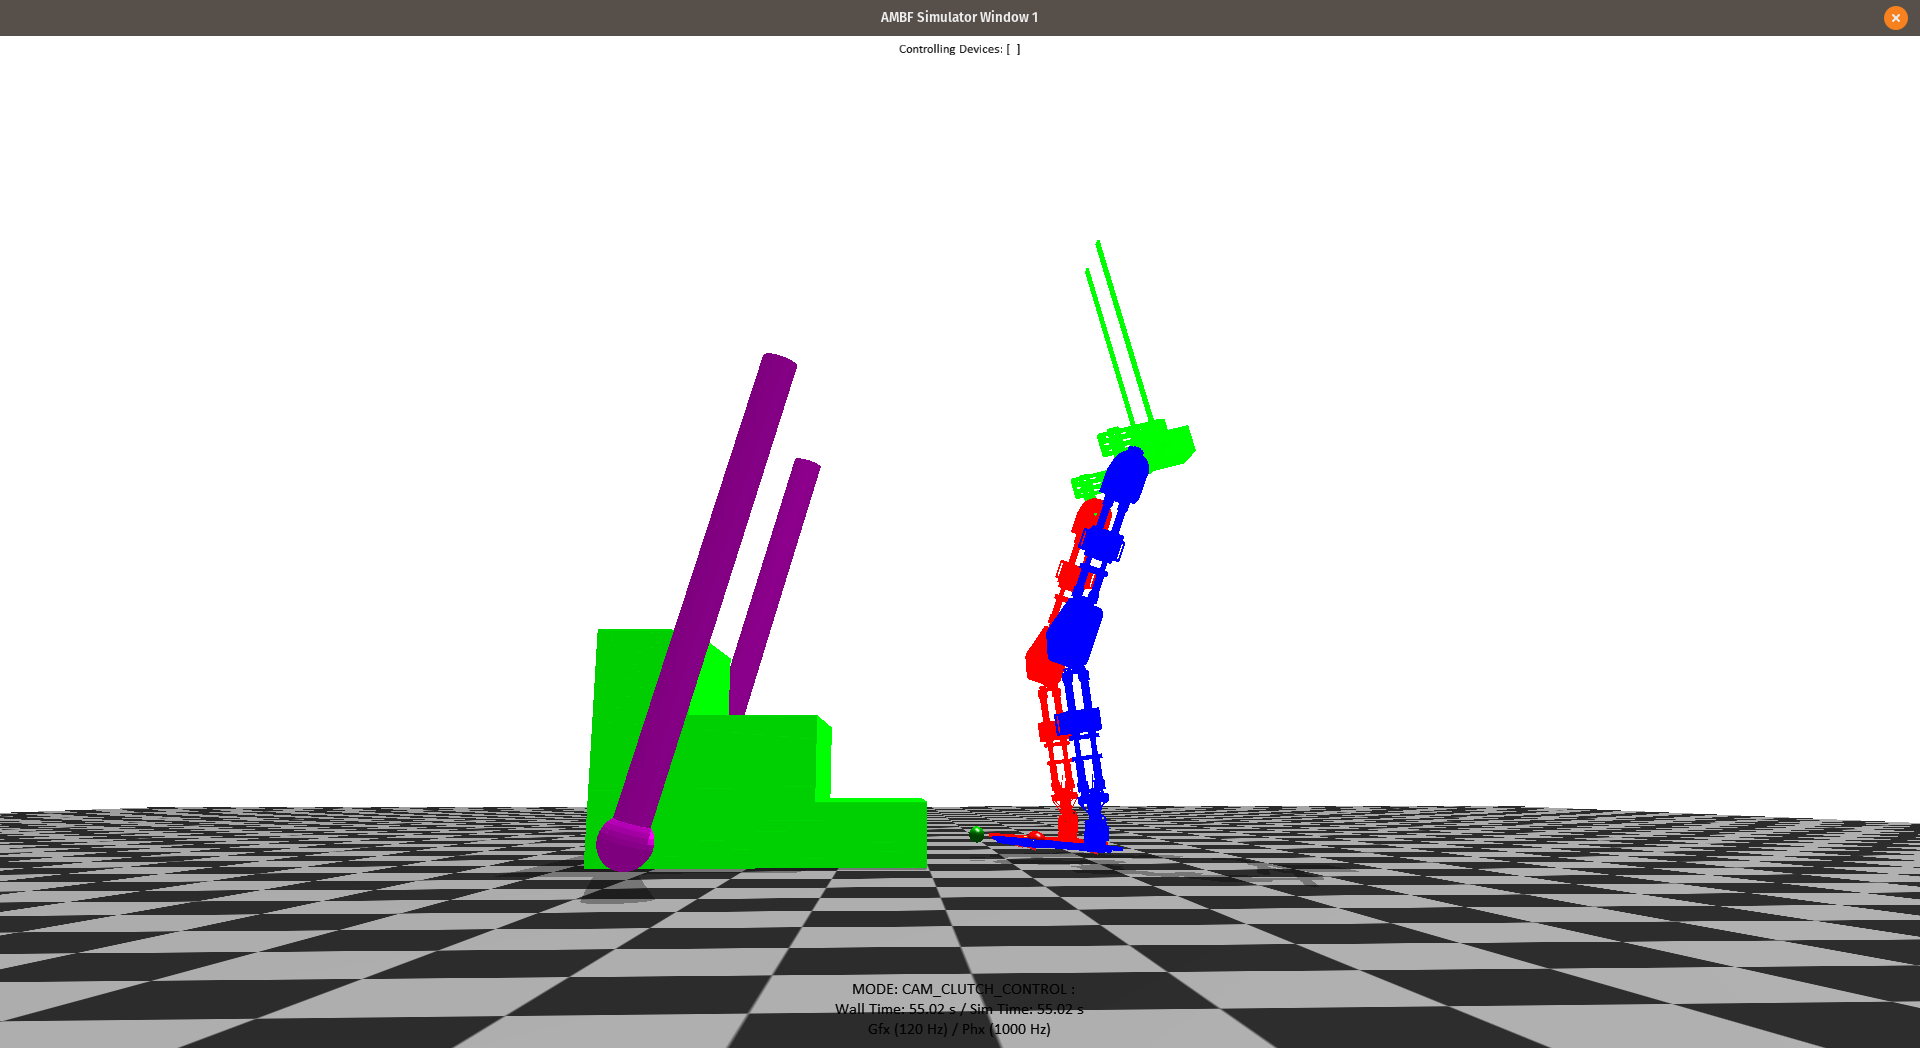
\includegraphics[scale=0.1]{images/sim/stair2.png}
        \caption{LARRE and the stair case in AMBF}
        \label{fig:exostair}
        \label{fig:sub1}
    \end{subfigure}%
    \begin{subfigure}{.5\linewidth}
       \centering
        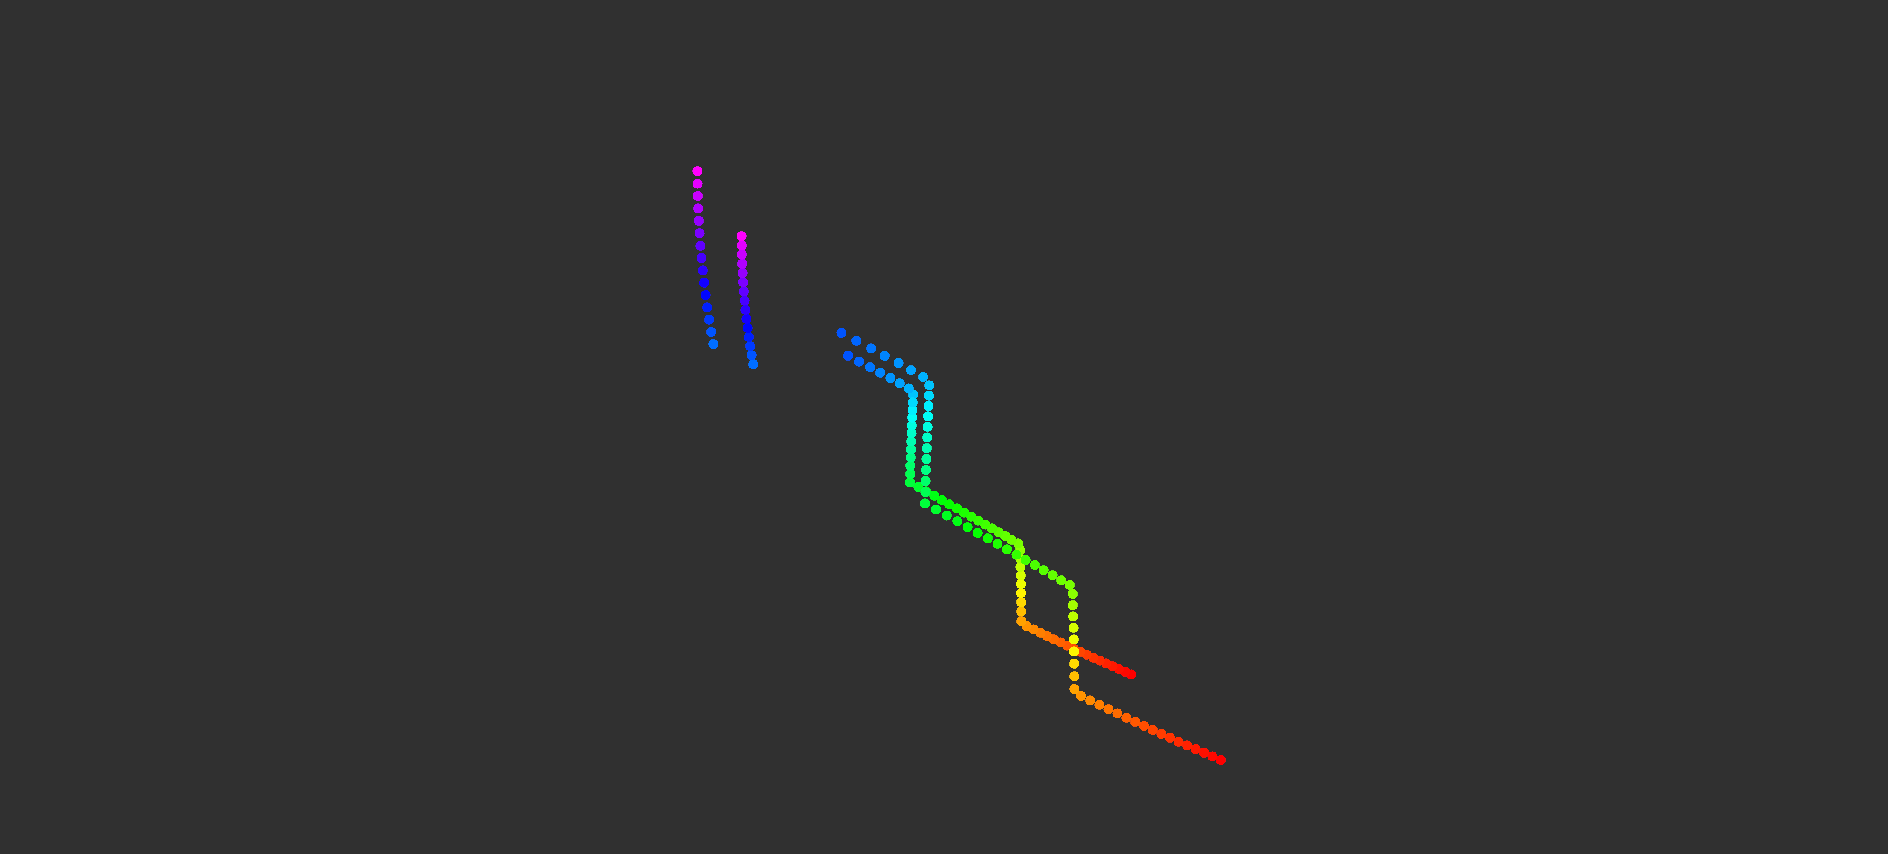
\includegraphics[scale=0.15]{images/sim/point_cloud_stairs.png}
        \caption[Point Cloud of the Stairs]{Point cloud of the stair as captured by LARRE}
        \label{fig:LIDAR}
        \end{subfigure}\\[1ex]
    \begin{subfigure}{\linewidth}
        \centering
        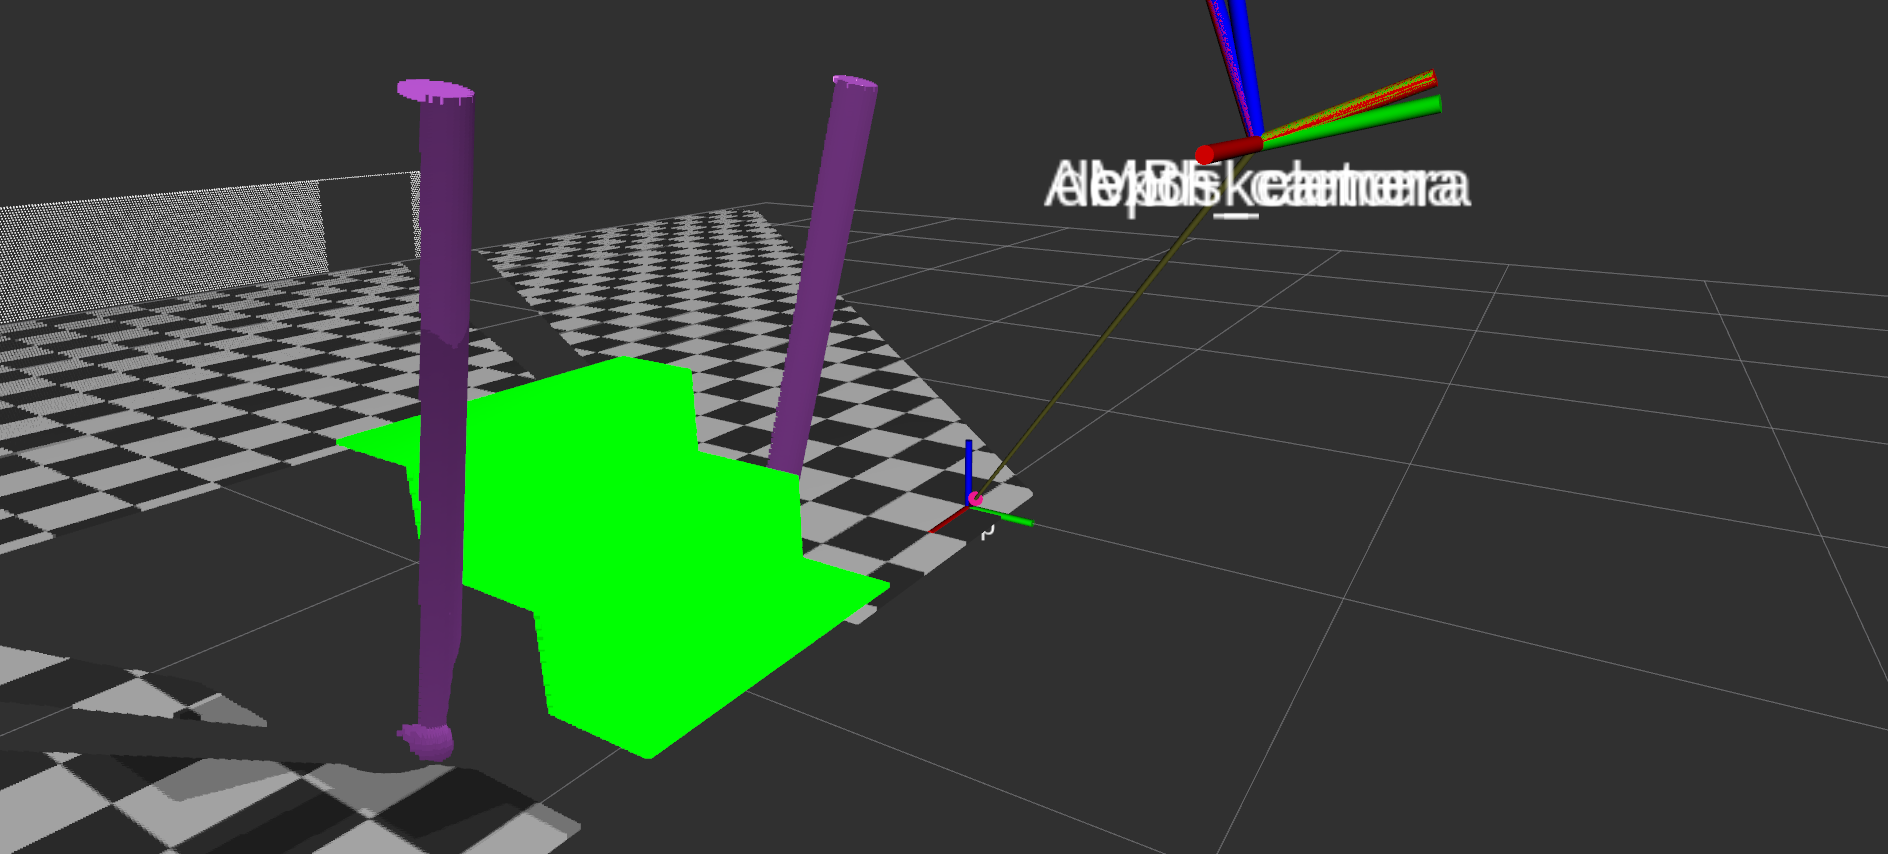
\includegraphics[scale=0.15]{images/sim/point_cloud_stairs2.png}
        \caption{Point cloud of the stair as captured by LARRE}
        \label{fig:DEPTH}
    \end{subfigure}
   \caption[LIDAR built into LARREs hip]{LARRE has built in LIDAR sensor to detect objects in the environment.}
   \label{fig:sensors}
\end{figure}
 
 
 
 \section{AMBF Control Architecture}
 \label{sec:controlarchitecture}
 
 \subsection{Overview}
 The controller architecture was developed with Shreyas Chandra Sekhar and presented a late-breaking result at iros 2021. Open source development of surgical robotic platforms as seen a lot of development in recent years with the development with the development of Collaborative Robotics Toolkit (CRTK)\cite{su2020collaborative}, da Vinci Research Kit \cite{d2021accelerating}, and AMBF The progress and development of these systems allow for researchers to develop new tools for surgical applications. The development of the  AMBF simulation platform allows for simulation of various surgical robotic platforms. 

The dynamics of the robots used in the medical or industrial applications are often complex, and may involve some redundant links and joints such as the dVRK robot\cite{wang2019convex}. Analytically calculating the dynamics model for a controller is complex and may lead to model singularities and errors that cause instability in the controller. This process is often very robot-specific as well. A model configuration file that allows for procedural generation of the dynamic model will ensure that the controller has a matching model for canceling out the non-linear dynamic errors of the robotic model.

These new simulation platforms presents the need for a open source control toolbox to interact and control the robotic platforms. This is split into two separate systems: a dynamics server, and a controller server. The dynamics server calculates the dynamics and kinematic properties of the robot. The controller server is used for calculating control commands for the robot. By dividing the implementation these two systems they can be used either together or separately.  Wrapping these system in ROS, the dynamics server can be accessed cross-platform and allows for a custom controller that incorporates dynamics of arbitrary robots to be readily implemented. Additionally, a control package is presented that leverages the dynamic server to implement the custom controller. This software architecture enables model-based controllers to be developed for, and evaluated on, different simulation and physical systems.  The dynamic server and controllers make up the \textit{ambf\_control\_system} package. While this tool is contrains \textit{ambf} in its name it can be used with any simulation system, in this paper we will only present the system application in AMBF. \autoref{fig:ambfcontrolartecture} shows a architecture diagram of the package. 
 

 

 \begin{figure}
     \centering
     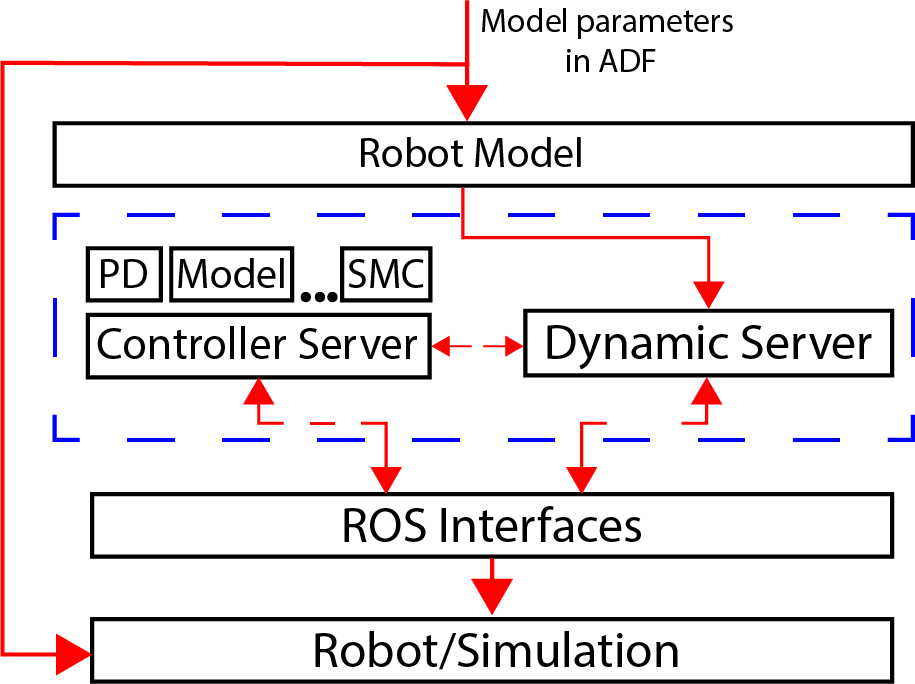
\includegraphics[scale=1.5]{images/software/dynamic_server_daigram.png}
     \caption[Controller package Diagram]{Architecture for control package}
     \label{fig:ambfcontrolartecture}
 \end{figure}
 
 

% \begin{table}[h]
%     \centering
%     \large
%  \begin{tabular}{||c | c ||} 
%  \hline
%   & Value (Hz)  \\ [0.5ex] 
%  \hline\hline
%  min & 98.54 \\ 
%  \hline
%  max & 5497.08  \\
%  \hline
%  mean & 520.27  \\
%  \hline
%  std & 184.92  \\ [1ex]
%  \hline
%  \hline
% \end{tabular}
%     \caption{Frequency of the Controller}
%     \label{tab:controlHist}
% \end{table}


 
 
 
 
 \subsection{Dynamic Server}
 The dynamic server is responsible for calculating the dynamics of the model for use in dynamic controllers and uses The Rigid Body Dynamics Library (RBDL)\cite{Felis2016}. The RBDL library is an open-source library for generating model dynamics for 3D objects. The RBDL library is based on the Featherstone spatial algebra methods. The RBDL library offers comprehensive methods to calculate the forward dynamics, inverse dynamics, and the robotic system's Jacobians. This library has been used to calculate the dynamics of human and exoskeleton motion to model the torque and force \cite{millard2017predicting} \cite{harant2017parameter}. Manns \textit{et. al} used RBDL to model interactions force between the human and exoskeleton \cite{manns2017motion}. 
 
 The dynamic server will parse the YAML file generated by the Blender ambf\_addon into an RBDL model. The server can handle multiple robot configurations by mapping a unique name to the RBDL model; this allows the server to handle multiple robots in the simulation. 
 The dynamic server is an abstraction layer between the RBDL API and the AMBF clients. The RBDL API provides the functionality to calculate the dynamics and kinematics of the system. The dynamics of the robotic system can be generalized in  \autoref{eq:motion}. $H(q)$ is the mass-inertia matrix, $C(q,\Dot{q})$ are the non-linear terms, $\tau$ is the torque,  $G(q)$ is the contact Jacobian, and $\lambda$ are the external force. \autoref{fig:DynCommunicationHistogram} shows the timing histogram for one million calls to the dynamic server. On average, the call timing was $0.49ms$ with a standard deviation of $0.07ms$.  


 \begin{figure}
     \centering
     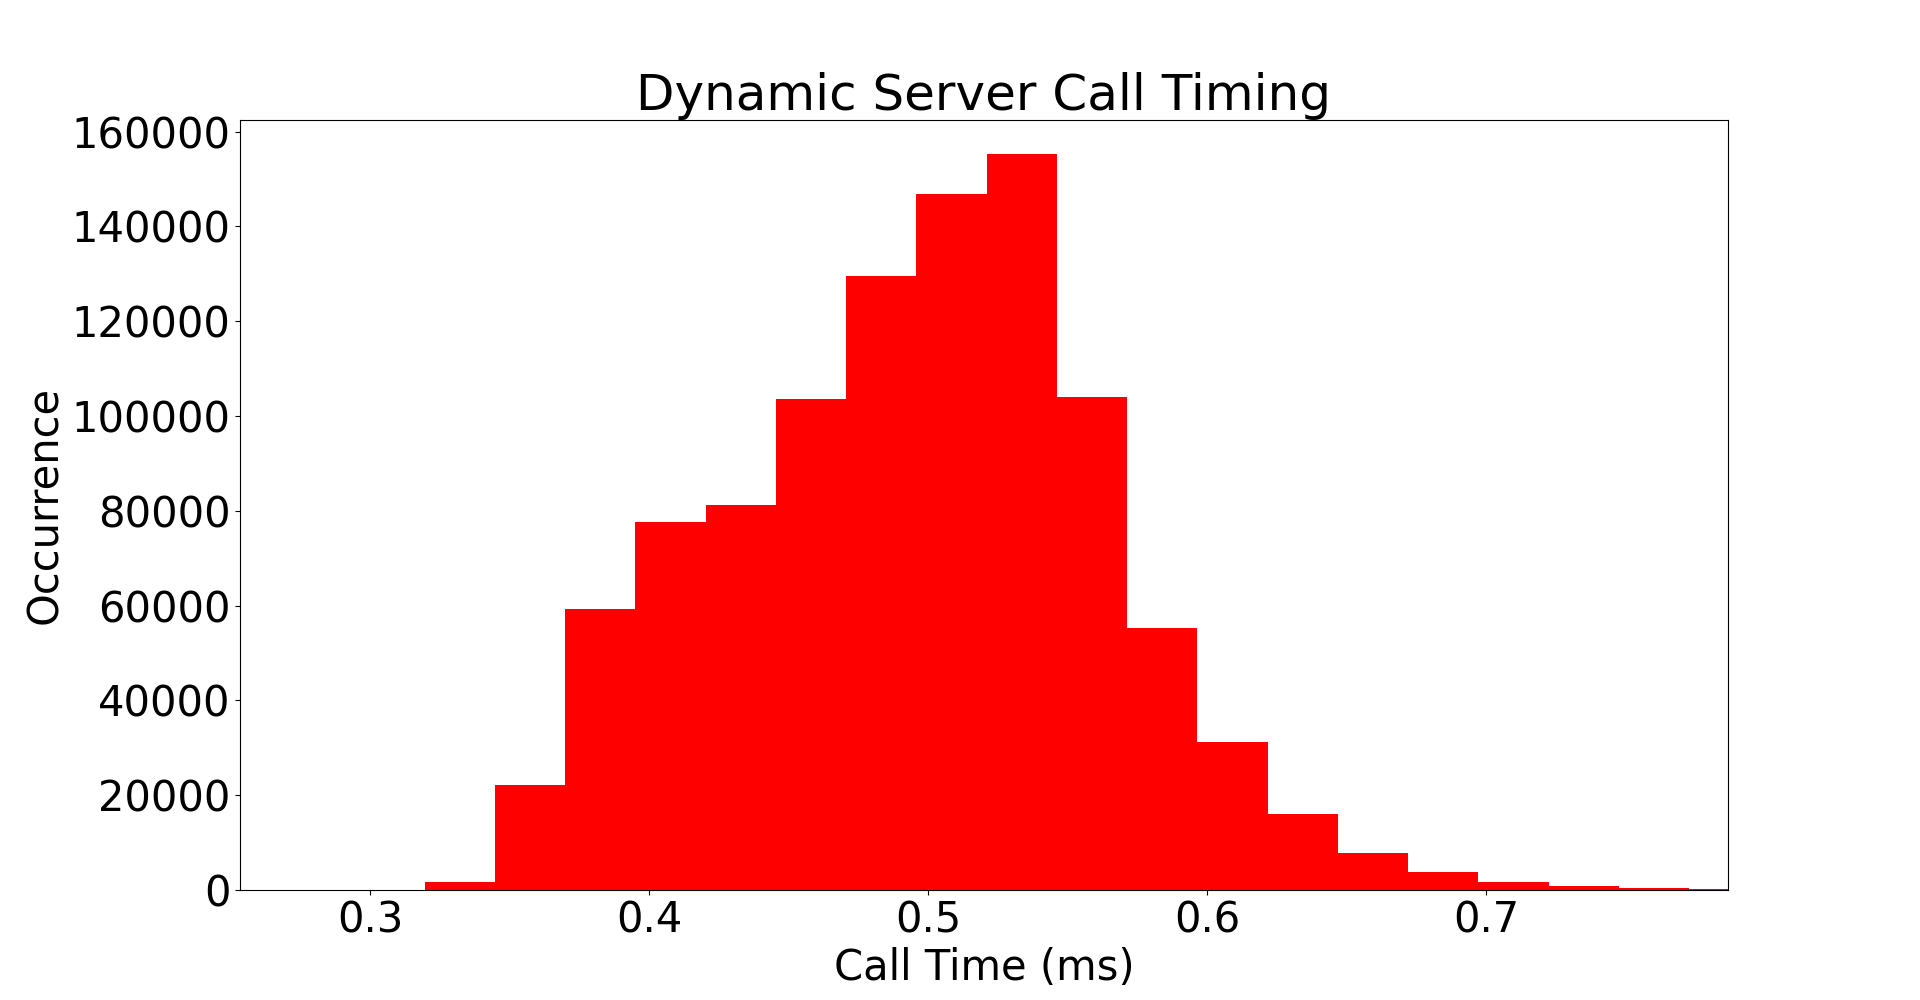
\includegraphics[scale=0.35]{images/software/dyn_loop_timing.png}
     \caption[Dynamic Timing Histogram]{Communication Timing Histogram for the Dynamics server}
     \label{fig:DynCommunicationHistogram}
 \end{figure}
 


\begin{equation}
\Large
    H(q) \Ddot{q} + C(q,\Dot{q}) = \tau + G(q)^T \lambda
    \label{eq:motion}
\end{equation}



The dynamic server is designed to be used with Python and C++ clients. This modality is achieved by wrapping the RBDL API in ROS services; this includes Jacobians, forward dynamics, inverse dynamics, and forward kinematics. These calculations have their own custom ROS service message that passes the necessary parameters down to the RBDL API and returns the calculated response. 

The AMBF client gathers the joint position ($q$), joint velocity ($\Dot{q}$), and acceleration ($\DDot{q}$) of the robot.  The forward kinematics are calculated using these variables as shown in \autoref{eq:FD}; this returns the torque at each of the joints. To find the joint acceleration, the joint position and velocity are required in addition to a torque or command ($\tau$) shown in \autoref{eq:ID}.  

\begin{equation}
    \Large
    \tau = ID(q,\Dot{q}, \Ddot{q})
    \label{eq:ID}
\end{equation}


\begin{equation}
    \Large
    \Ddot{q} = FD(q,\Dot{q}, \tau )
    \label{eq:FD}
\end{equation}



\autoref{fig:DynCommunicationHistogram} shows the average time to get and receive a message from the dynamic server. The server was called one million times resulting in an average call time of $0.49ms$ with a standard deviation of $0.07ms$. Calling the RBDL API directly takes approximately $0.013ms$. While, this is a magnitude more it is still under $1ms$ of time. This trade should be acceptable for the modality that the dynamic server provides. 


 
 
 \subsection{Control Server}
 
 The controller manager is responsible for managing the controllers and calculating the control commands. The control manager is split into two systems; the controllers and manager that pass the commands into the desired controller. 
\autoref{fig:CntrlCommunicationHistogram} shows the timing histogram for one million calls to the controller server; on average, the call timing was $0.51ms$ with a standard deviation of $0.043ms$.  

 \begin{figure}
     \centering
     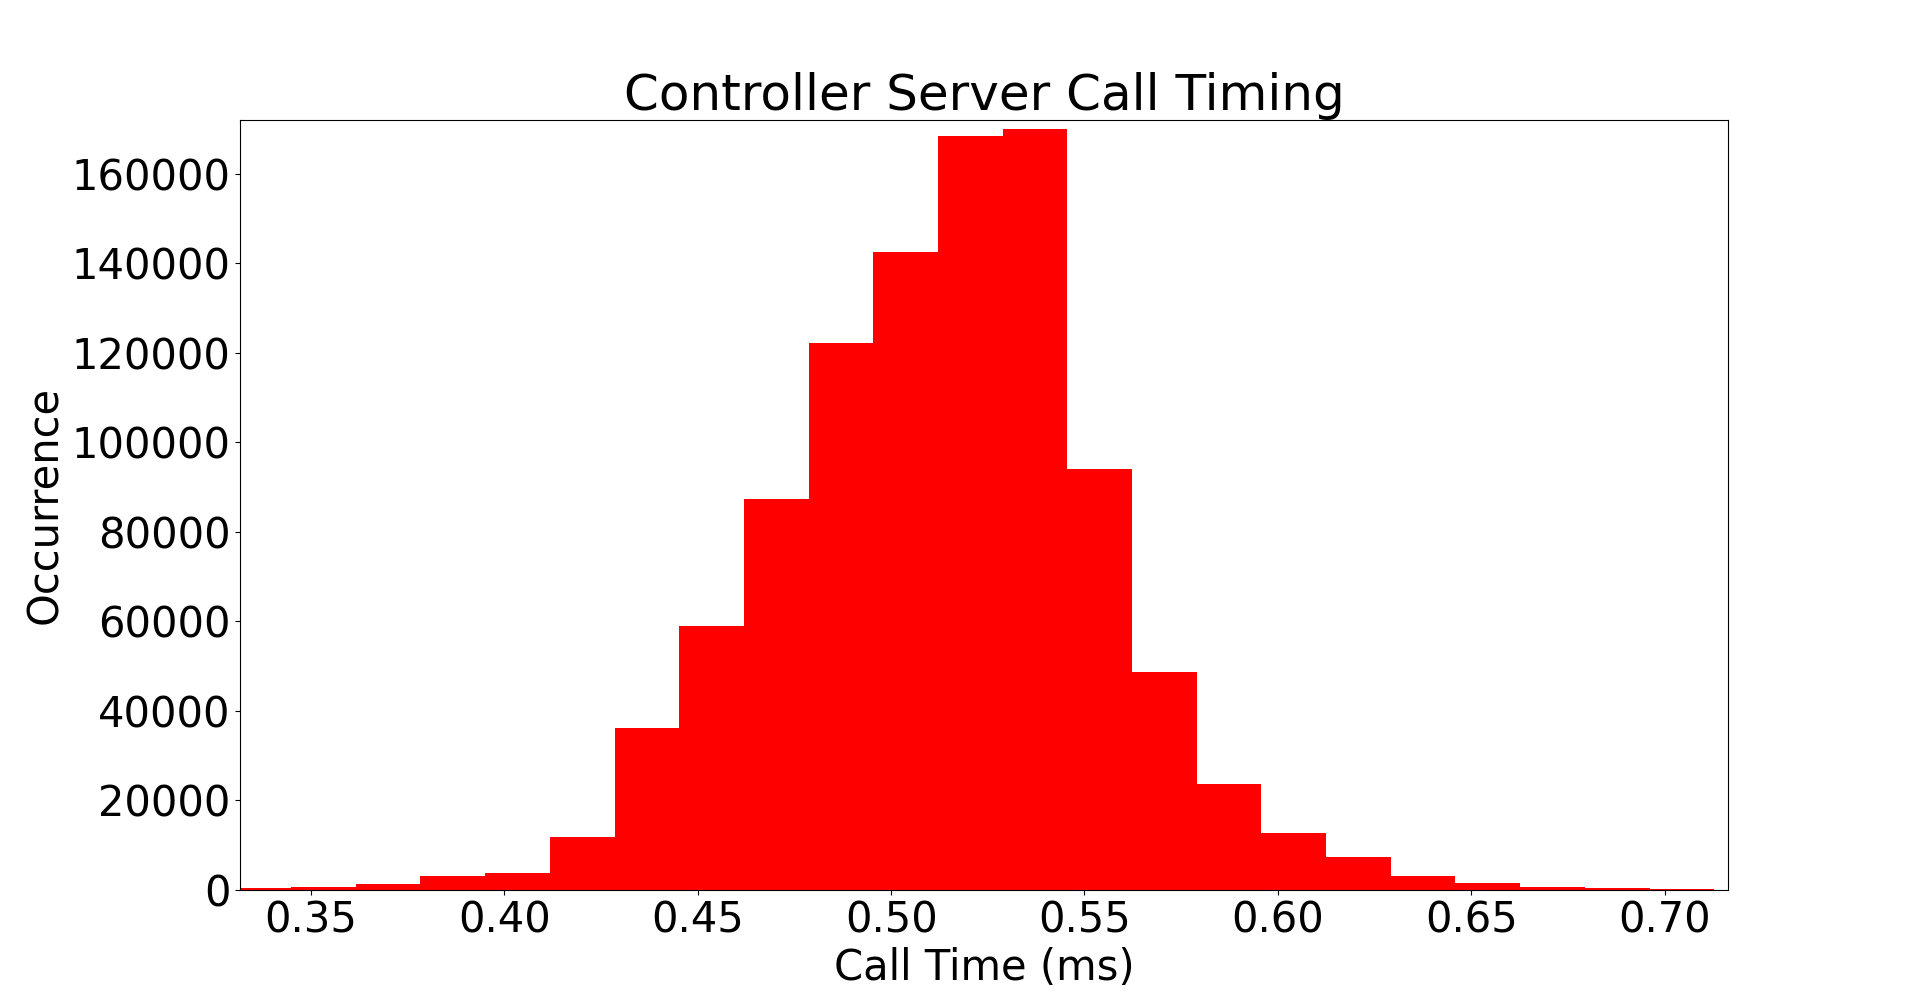
\includegraphics[scale=0.35]{images/software/control_loop_timing.png}
     \caption[Controller Server Timing Histogram]{Communication Timing Histogram for the Controller Server}
     \label{fig:CntrlCommunicationHistogram}
 \end{figure}


The control manager is a ROS service that abstracts the command inputs and allows for communication between the user and the desired controller; this allows the manager to be accessed from the Python or C++ application using a ROS service call. The control manager does not directly interact with the AMBF simulation environment. It is solely responsible for passing the control parameters back and forth between the user and the controller. This framework requires the user to maintain the control loop, gather the robot state, and send the control commands down to the robot. A basic control diagram is shown in \autoref{fig:Basic_AMBF_Control_Loop}.


\begin{figure}[h!]
    \centering
    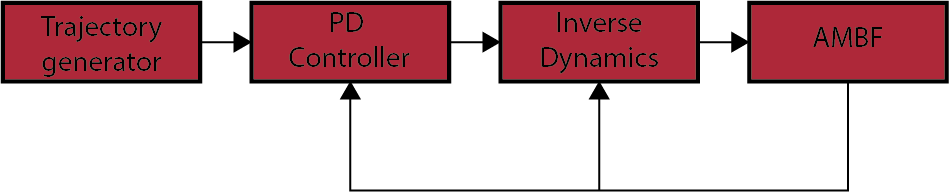
\includegraphics[scale=1.25]{images/sim/control_outline.png}
    \caption[Basic AMBF Control Loop]{Basic AMBF Control Loop}
    \label{fig:Basic_AMBF_Control_Loop}
\end{figure}

Controllers are attached to the manager and are accessed at run time by the user. Multiple controllers can be connected to the manager, and each controller has a unique name to identify it.  A controller can be designed to collect external data via topics for obstacle avoidance or other external information. This framework is achieved by having each controller extend the \textit{BaseController} class, which acts as a base class to develop the controller. This framework allows for flexibility in the design of a controller. Several controllers are built into the package, including a PD controller, a model-based controller, and gravity compensation controller.  



\section{Integration of Control Architecture}

\autoref{fig:SystemDiagram} shows a diagram of how all the systems are connected. The red objects are a part of the \textit{ambf\_control\_system} package, the green objects are part of the \textit{ambf} package, the gray objects are external systems or files, and the round objects depict ROS nodes. ROS is utilized as the primary communication method between the different systems.

  \begin{figure}[h]
    \centering
    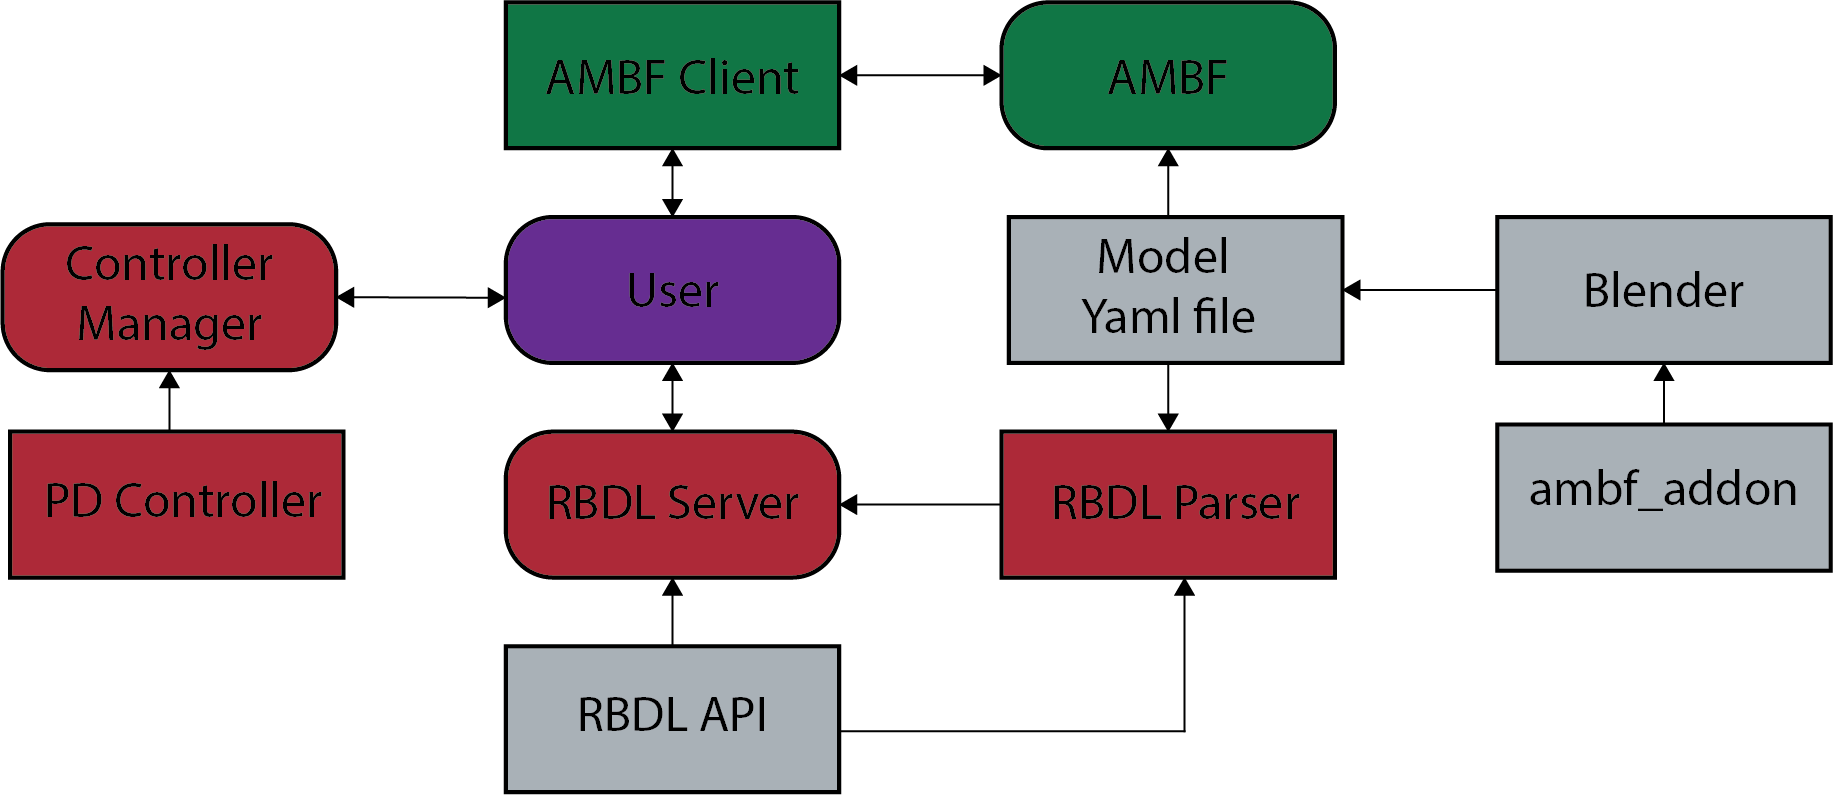
\includegraphics{images/sim/AMBF_control_diagram (1).png}
    \caption[AMBF Control Diagram]{Control diagram and connections between the separate systems. \textit{ambf\_control\_system} package work directly with the \textit{ambf} system. The configuration of the robotic system is defined in Blender and saved into a YAML file.}
    \label{fig:SystemDiagram}
\end{figure}

 
 The AMBF Python client allows for access to the joint's kinematics and dynamics. The control loop for LARRE is designed to run at $500Hz$ managed by a ROS timer. The internal state is updated in each cycle, and a torque command is sent to the model. These operations should occur approximately every $2ms$. The loop timing was measured over a $60s$ period to measure the loop's efficiency. \autoref{fig:CommunicationHistogram} shows the distribution of the control timing with the average timing of the loop being $1.99ms$ with a standard deviation of $0.29ms$, which is within an acceptable margin for the simulation purposes. 
 
  
 \begin{figure}
     \centering
     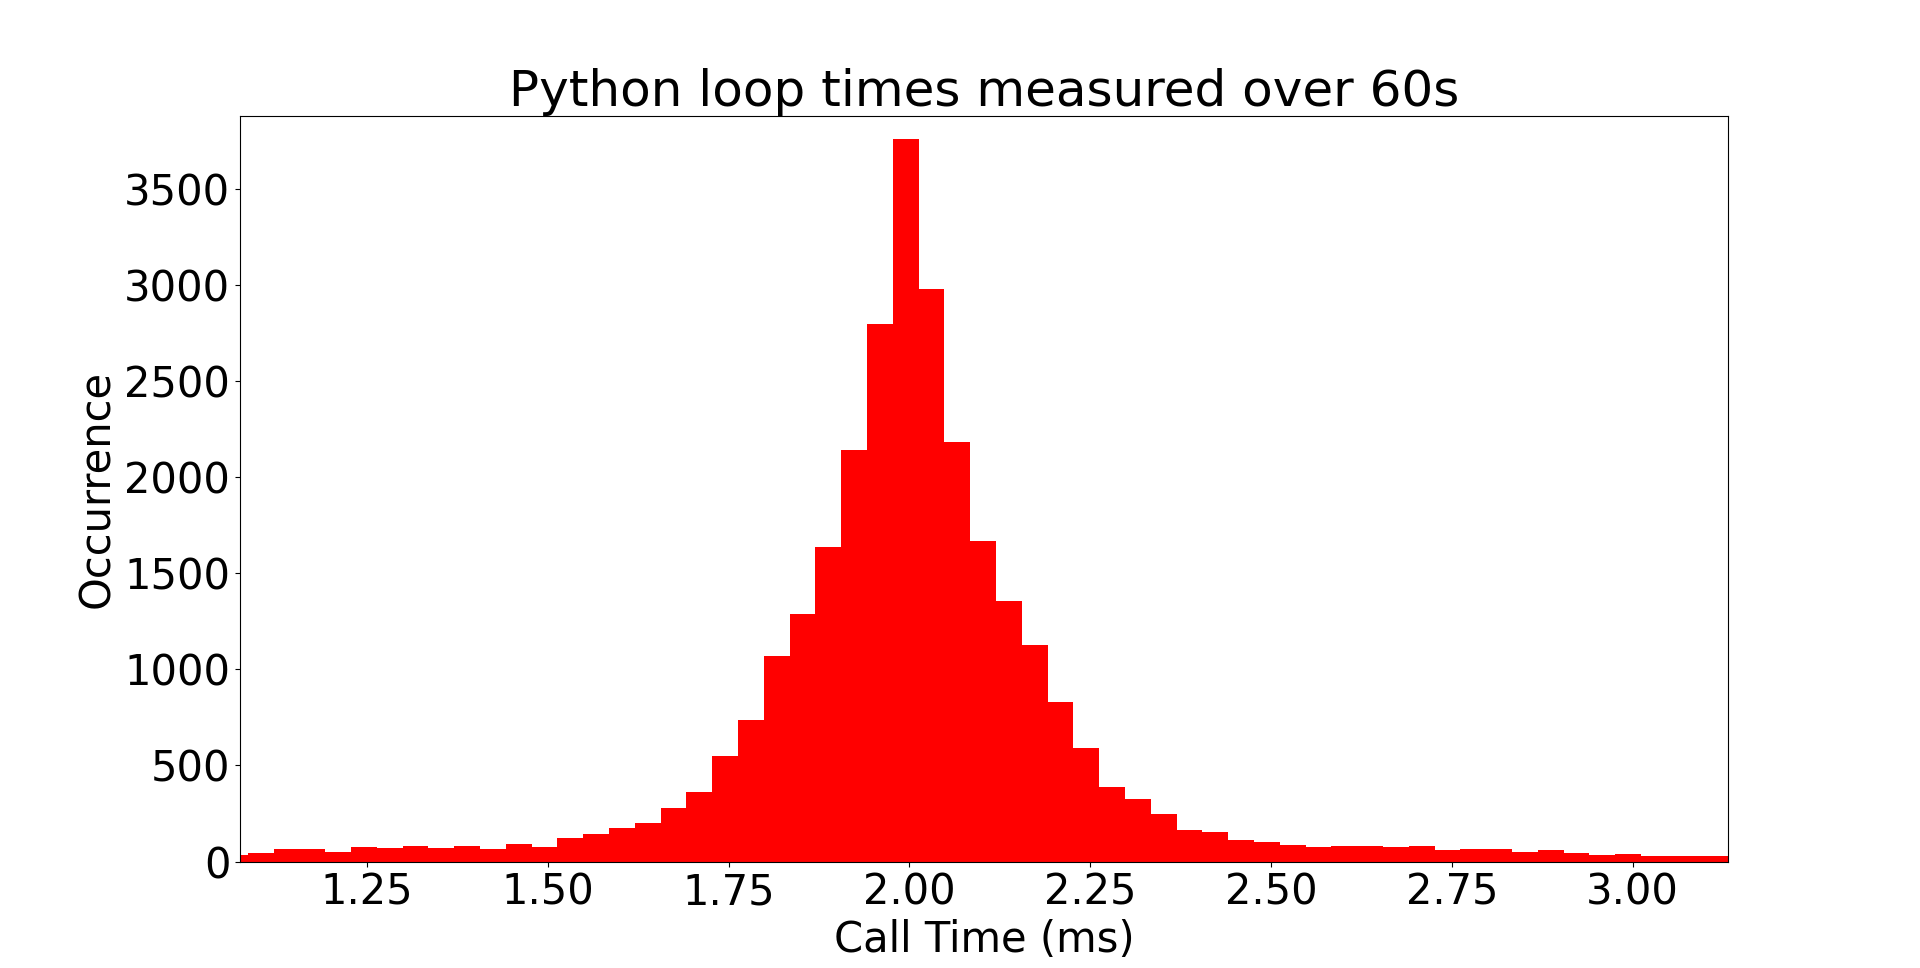
\includegraphics[scale=0.35]{images/sim/loop_timming.png}
     \caption[Communication Timing Histogram]{Communication Timing Histogram}
     \label{fig:CommunicationHistogram}
 \end{figure}
 


\section{Contributions}

The AMBF simulation framework provides a well-structured environment for the testing of robotic systems. The functionality of the package was enhanced with the development of the \textit{ambf\_control\_system} package. This package enables a dynamic controller to be built to control the AMBF models. By developing an AMBF to RBDL parser, the dynamic control model is identical to the simulation model. By abstracting the RBDL calculations and creating the model, it can be accessed by either Python or C++ AMBF applications. The control architecture allows for controllers to be designed and implemented. Attaching the controller to the control manager allows the controller to be accessed by a ROS service call. This package provides a comprehensive method of developing controllers for AMBF robots. This control package was released open-source for community use and development alongside AMBF, creating a total package for simulating and controlling robotic systems.   

The simulation framework and newly developed control architecture allow for custom controllers to be built and tested to control LARRE. It models the interaction between the human and exoskeleton. The joint sensors provide state feedback enabling trajectory control by having both the human and exoskeleton joints controllable and a cooperative controller to be developed and tested in the simulation. Other simulation frameworks do not allow for such applications to be tested. More development and testing needs to be conducted in order to get ground level walking working. This includes fixing the friction properties of LARRE feet and inserting force sensors into the feet in order to detect each step of the exoskeleton. This should be possible as the AMBF platform grows as more researchers use and develop on the platform. AMBF in its current state makes it very difficult to implement this required changes.   


% The control input was measured over one million iterations to measure the execution time. The total time to call the control server and RBDL server is $1.53ms$; this includes sending and receiving both messages to both servers. Individually the calculation of the inverse kinematics is $0.013ms$, while the controller calculation takes $0.024ms$.  A direct call to the RBDL API is faster than calling it with the abstraction layer, which increases the total time required to calculate the control command. However, the abstraction layer adds the benefits of allowing cross-language support and eliminates the need to develop a YAML to RBDL parser for C++ and Python, which would double the amount of code that has to be developed and maintained. The trade-off for eliminating these complications is a time penalty for calling the ROS service of approximately $1ms-1.5ms$. This time loss is acceptable for the trade-off in the gained functionality. 






 
 
%  This control package was made modular to control any serial link or parallel link manipulator modeled in AMBF. This package called the \textit{ambf\_control\_system} package consists of a dynamic server and a controller server. The dynamic server is used to calculate the dynamics of the robotic model. The controller server provides APIs to develop and manage custom controllers. 
 
 
%  The dynamics of the robots used in the medical or industrial applications are often complex, and may involve some redundant links and joints such as the dVRK robot\cite{wang2019convex}. Analytically calculating the dynamics model for a controller is complex and may lead to model singularities and errors that cause instability in the controller. This process is often very robot-specific as well. A model configuration file that allows for procedural generation of the dynamic model will ensure that the controller has a matching model for canceling out the non-linear dynamic errors of the robotic model. 
 
%  The contribution of this package is that it allows the dynamics of any model defined in the \textit{ADF} to be generated. It is not exclusively used for simulating systems in AMBF; it can also be used for generating the dynamics of robotic systems being simulated in Gazebo \cite{koenig2004design} or physical systems. 
 

%  Additionally, it expands the usability of AMBF by providing a comprehensive software package to control the AMBF simulation models. The package is split into two parts, a dynamics model server parsing configuration files and calculating the robot's dynamics and a controller interface for designing and implementing custom controllers. \autoref{fig:ambfcontrolartecture} shows a architecture diagram of the package. 